%%%%%%%%%%%%%%%%%%%%%%%%%%%%%%%%%%%%%%%%%%%%
% Submitted Abstract

%The deep chlorophyll maximum (DCM) is a well known feature of the global ocean. However, its description and the study of its formation are a  challenge, especially in the peculiar environment that is the Black Sea. The retrieval of chlorophyll a (Chla) from fluorescence (Fluo) profiles recorded by biogeochemical-Argo (BGC-Argo) floats is not trivial in the Black Sea, due to the very high content of colored dissolved organic matter (CDOM) which contributes to the fluorescence signal and produces an apparent increase of the Chla concentration with depth.

%Here, we revised Fluo correction protocols for the Black Sea context using co-located in-situ high-performance liquid chromatography (HPLC) and BGC-Argo measurements. The processed set of Chla data (2014–2019) is then used to provide a systematic description of the seasonal DCM dynamics in the Black Sea and to explore different hypotheses concerning the mechanisms underlying its development.

%Our results show that the corrections applied to the Chla profiles are consistent with HPLC data. In the Black Sea, the DCM begins to form in March, throughout the basin, at a density level set by the previous winter mixed layer. During a first phase (April-May), the DCM remains attached to this particular layer. The spatial homogeneity of this feature suggests a hysteresis mechanism, i.e., that the DCM structure locally influences environmental conditions rather than adapting instantaneously to external factors.

%In a second phase (July-September), the DCM migrates upward, where there is higher irradiance, which suggests the interplay of biotic factors. Overall, the DCM concentrates around 45 to 65% of the total chlorophyll content within a 10 m layer centered around a depth of 30 to 40 m, which stresses the importance of considering DCM dynamics when evaluating phytoplankton productivity at basin scale.

%%%%%%%%%%%%%%%%%%%%%%%%%%%%%%%%%%%%%%%%%%%%

\documentclass[final]{beamer}
%% Possible paper sizes: a0, a0b, a1, a2, a3, a4.
%% Possible orientations: portrait, landscape
%% Font sizes can be changed using the scale option.
\usepackage[size=a0,orientation=landscape,scale=1.25]{beamerposter}
\usetheme{ARTMAN_PERSEUS}
%\usetheme{LLT-poster}
%\usecolortheme{ComingClean}
%\usecolortheme{Entrepreneur}
%\usecolortheme{ConspicuousCreep}  %% VERY garish.

\usepackage[utf8]{inputenc}
\usepackage[T1]{fontenc}
\usepackage{libertine}
\usepackage[scaled=0.92]{inconsolata}
\usepackage{hyperref}

\newcommand{\ExternalLink}{%
    \tikz[x=1.2ex, y=1.2ex, baseline=-0.05ex]{% 
        \begin{scope}[x=1ex, y=1ex]
            \clip (-0.1,-0.1) 
                --++ (-0, 1.2) 
                --++ (0.6, 0) 
                --++ (0, -0.6) 
                --++ (0.6, 0) 
                --++ (0, -1);
            \path[draw, 
                line width = 0.5, 
                rounded corners=0.5] 
                (0,0) rectangle (1,1);
        \end{scope}
        \path[draw, line width = 0.5] (0.5, 0.5) 
            -- (1, 1);
        \path[draw, line width = 0.5] (0.6, 1) 
            -- (1, 1) -- (1, 0.6);
        }
    }
    
\usepackage{enumitem}
\usepackage{filecontents}

\usepackage{natbib}
\bibliographystyle{mnras}

\renewcommand{\bibsection}{}

\graphicspath{{./figs/}
  {./figs/logo/}
}

\newcommand{\unit}[1]{$\mathrm{#1}$}

\setbeamertemplate{bibliography entry article}{}
\setbeamertemplate{bibliography entry title}{}
\setbeamertemplate{bibliography entry location}{}
\setbeamertemplate{bibliography entry note}{}

%%%%%%%%%%%%%%%%%%%%%%%%%%%%%%%%%%%%%%%%%%%%%%%%%

\author[acapet@ulg.ac.be]{
Florian Ricour$^{1,2,*}$,
Arthur Capet$^{1,*}$,
Fabrizio D'Ortenzio$^{2}$,
Bruno Delille$^{1}$,
Marilaure Gr\'{e}goire$^{1}$}
\title[Ricour, F., Capet, A., D’Ortenzio, F., Delille, B. and Grégoire, M., 2021, \textit{Biogeosciences}, 18(2), 755–774. \vspace{2cm} \href{https://bg.copernicus.org/articles/18/755/2021/}{\color{red} \Large \ExternalLink}]
{Deep Chlorophyll Maximum Dynamics in the Black Sea}
%

\institute{
  $^1$ FOCUS, Liège University, Belgium,
  $^2$ Laboratoire d'Oc\'{e}anographie de Villefranche, Sorbonne Universit\'{e}s, France}
  
% Optional foot image
% \footimage{           
\includegraphics[width=9cm]{mast.png}
%            \vspace{1cm}
%                       \includegraphics[width=7cm]{uliege.jpg}
%            \vspace{3cm}
%             }

\begin{document}
  \begin{frame}[fragile]\centering
    \begin{columns}[T]

      %%%%%%%%%%%%%%%
      % LEFT COLUMN %
      %%%%%%%%%%%%%%%   
      
      \begin{column}{.33\textwidth}
%	\section{Context \& Method}
%	\subsection{Deep Chlorophyll Maximum}
	%%% CONTEXT
	\begin{alertblock}{Research Objectives}
	\justify
	
The presence of a subsurface layer of maximum chlorophyll (Chl) concentration, or deep chlorophyll maximum (DCM), is a widespread feature of the world ocean \citep{Cullen2015}, but the mechanisms of its formation and maintenance are still under debate.\\
\vspace{5mm}

Common understanding involves instantaneous factors, such as maximum growth resulting from a compromise between light and nutrient limitations.
More recently, \citet{Navarro2013} argued that the DCM is conditioned by the history of the bloom, and emerges in spring at a density corresponding to that of the winter mixed layer.\\
\vspace{5mm}

This second understanding depicts the DCM as a self-preserving structure that remains at a near constant density layer by preventing upward nutrient fluxes and downward light penetration. It would explain why chlorophyll profiles from the global temperate ocean and the Mediterranean Sea are stable on a density scale while their depth is highly variable.\\
\vspace{5mm}

The peculiarities of the open Black Sea environment, i.e. its strong and stable stratification and relatively low water transparency, make it an interesting site to study DCM dynamics and to confront these two understanding of the DCM dynamics. 
\end{alertblock}
	
\begin{block}{Method}
We use BGC-Argo data (2014–2019, ca. 1000 profiles) to characterize the vertical distribution of Chl in the Black Sea. The processing of raw fluorescence involved:
\begin{itemize}[wide, labelwidth=!,labelindent=0pt, label=$\diamond$]
    \item applying a static sensor correction \citep{Roesler2017};
    \item a correction for CDOM fluorescence based on deep fluorescence \citep{Xing2017};
    \item correcting surface values for non-photochemical quenching  \citep{Xing2012}
\end{itemize} 
These procedures are validated on the basis of an HPLC in-situ profile.
\end{block}

%% CONCLUSIONS 
%\section{Conclusions \& Perspectives}
\begin{alertblock}{Conclusions}
	%  	  \vskip -5mm
%	  \begin{columns}[T]
%	    \begin{column}{.63\columnwidth}	  
\begin{itemize}[wide, labelwidth=!,labelindent=0pt, label=$\diamond$]
		    \item We stress the importance of considering DCM dynamics for assessments of Black Sea productivity, as it dominates Chla distribution from April to October.
	        \item  The hysteresis hypothesis \citep{Navarro2013} holds from April to May.
	        \item During a second phase (July-September), biotic factors are responsible for an upward displacement of the DCM structure.
	        \item On average, the DCM concentrates more than 50\% the total Chla content within a 10 \unit{m} layer centered at a depth of about 35 \unit{m}.  
	        \item HPLC datasets should be consolidated in the Black Sea for  BGC-Argo calibration.
	      \end{itemize}
	\end{alertblock}
	
	%% REFS
	\begin{block}{References}
	\vskip -5mm
	  \footnotesize
    \bibliography{biblio.bib}
	\end{block}
      \end{column}
      
      %%%%%%%%%%%%%%%%%
      % SECOND COLUMN % 
      %%%%%%%%%%%%%%%%%
      
      %%% RESULTS 
      \begin{column}{.64\textwidth}
%       \section{Results}
      

	%%%% COMP MODELS 
	\begin{block}{Morphology of Chl profiles}
	 % \vskip -12mm
	Chl profiles were classified in terms of best-matching analytic forms. 
	In addition, DCM profiles requires Chl concentration 30\% larger than surface Chl concentration.\\
	As no spatial patterns emerged across the central basin, the seasonality of DCM dynamics can be considered as spatially homogeneous in the Black Sea. 
	  \begin{columns}[T]
	  
	    \begin{column}{.32\textwidth}
	    \centering{\alert{Examples of Non-DCM profiles}}
	   	     \begin{figure}
     		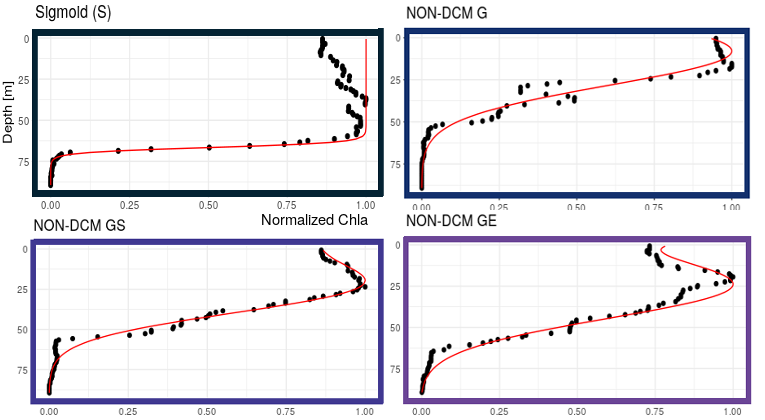
\includegraphics[width=.9\columnwidth]{figs/DCMforms_nonDCM.png}
		    \end{figure}
	    \end{column}
	    
	    \begin{column}{.32\textwidth}
	    \centering{\alert{ Monthly occurrences}}
	      \begin{figure}
     		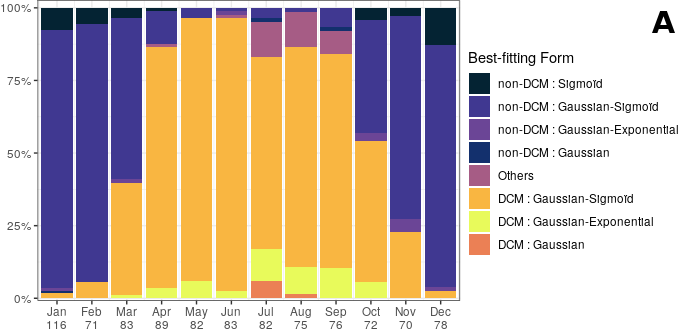
\includegraphics[width=\columnwidth]{figs/FIG3-G.png}
		    \end{figure}
	    \end{column}
	  
	    \begin{column}{.32\textwidth}
	       \centering{\alert{Examples of DCM profiles}}
	      	\begin{figure}
     		 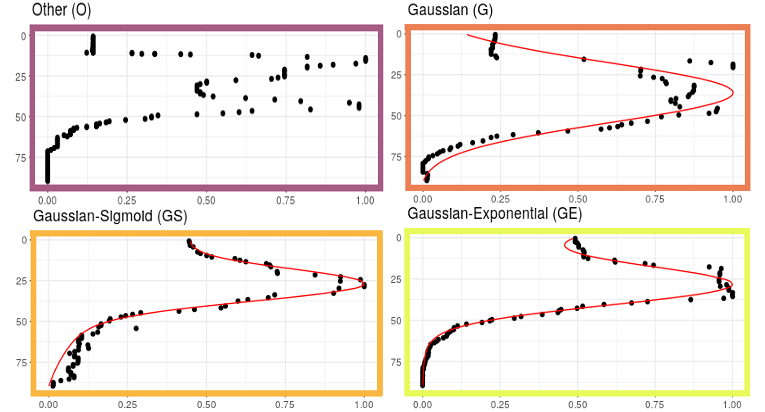
\includegraphics[width=.9\columnwidth]{figs/DCMforms_DCM.png}
		    \end{figure}
	    \end{column}	    
	  \end{columns}
	  
	\end{block}
	
	\begin{block}{ A DCM season in the Black Sea }
\vskip -12mm
	  \begin{columns}[T]
	    \begin{column}{.20\textwidth}
	    \subsection{Vertical coordinates}
	    We used three systems of vertical coordinates to characterize the DCM seasonal dynamics.
        \begin{itemize}[wide, labelwidth=!,labelindent=0pt]
          \item[\alert{Depth}] is used in BGC-Argo data.
          \item[\alert{Density}] is used in the Black Sea as  stratification strongly structures biogeochemical processes. 
          \item[\alert{PAR}] Using absolute irradiance, instead of the usual euphotic depth (1\% of surface PAR) makes more sense from a physiological point of view. 
        \end{itemize}

        \subsection{Horizons of Chl profiles}
        \begin{itemize}[wide, labelwidth=!,labelindent=0pt]
          \item[\alert{MLD}] The mixed layer depth is defined by a  density difference with respect to surface.
          \item[\alert{DCM}] The depth of the DCM is obtained as a parameter of the fitted analytical forms.
          \item[\alert{low}] The lower limit of Chl is identified as the lower depth with [Chl]>0.01 $\mathrm{mg\,m^{-3}}$.
          \item[\alert{50,bottom/top}] : The "bulk" of Chl content is defined as the smaller vertical range gathering 50\% of the vertically integrated Chl content. These horizons mark its lower and upper limits. 
        \end{itemize}

	    \end{column}
	    
	    \begin{column}{.33\textwidth}
		    \begin{figure}
     		    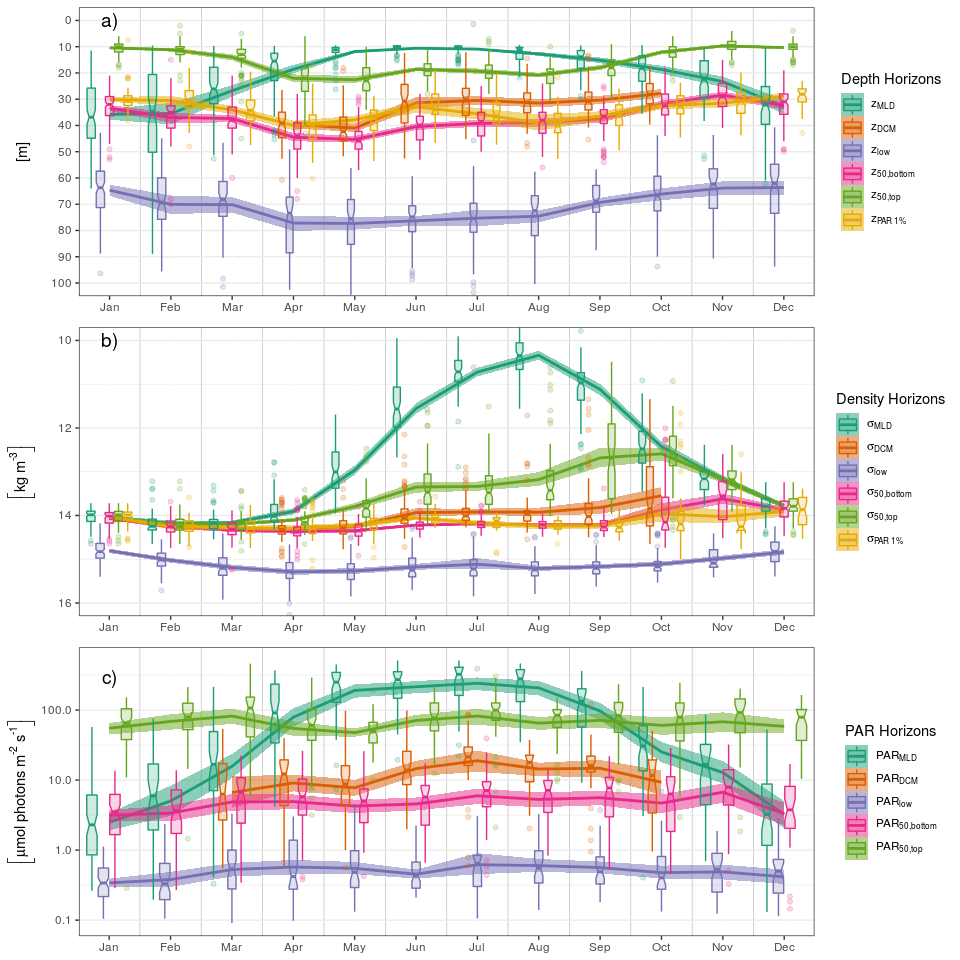
\includegraphics[width=\columnwidth]{figs/FIG5.png}
		    \end{figure}
		    \begin{figure}
     		    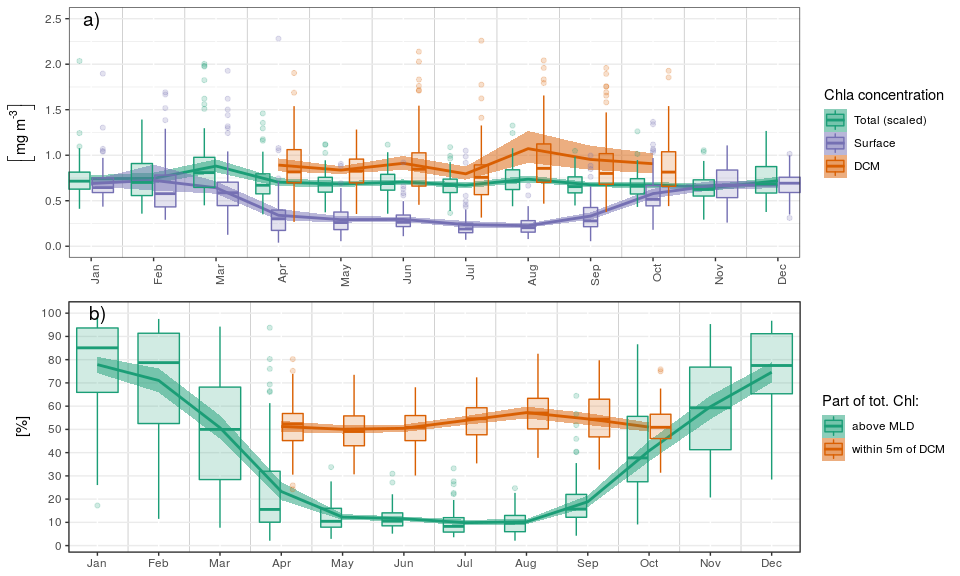
\includegraphics[width=\columnwidth]{figs/FIG6.png}
		    \end{figure}
	    \end{column}

	    \begin{column}{.42\textwidth}
	    \subsection{Seasonal phases}

\alert{In winter}, the MLD extends beyond the euphotic depth (\textbf{B}).
The DCM appears at the base of the MLD in March, in agreement with the general Sverdrup theory.\\

\vspace{5mm}
\alert{April–May} The DCM remains close to the density layer of winter MLD (\textbf{C}). A large spread in DCM depth on light and depth scales (A,C) suggests that density-driven factors sets the DCM depth. This is confirmed by the ratio $\sigma_{DCM}/\sigma_{winter MLD}$ obtained from individual profiles (\textbf{X}).\\

\vspace{5mm}
\alert{June-August} In June, the average Chl profile shifts towards a structure that remains stable through the summer. This shift involves :
\begin{itemize}[wide, labelwidth=!,labelindent=0pt, label=$\diamond$]
    \item hints of photoacclimation (particle  back-scattering data, not shown);
    \item appearance of Gaussian profiles (\textbf{A}),
and depletion of surface Chl;
   \item upward DCM displacement on both depth and pycnal scales
(\textbf{B,C}),
   \item upward DCM displacement on the irradiance scale (\textbf{D}),
   \item a decrease in the spread of irradiance values at the DCM,  
   \item an increase of Chl content around the DCM (\textbf{F}).
\end{itemize}
 This shift opposes the response expected from increased surface incoming irradiance and reduced nutrient upward flux, which suggest strong contribution of biotic factors, such as phytoplantkon species succession \cite{Mikaelyan2018} and/or changes in grazing pressure. \\
 
\vspace{5mm}

\alert{In October}, end of the DCM season, the DCM evolves away from the density layer of the  winter MLD. A marked spatial gradient is denoted (\textbf{F}), suggesting an influence of lateral nutrient inputs. 
 
 		    \begin{figure}
     		    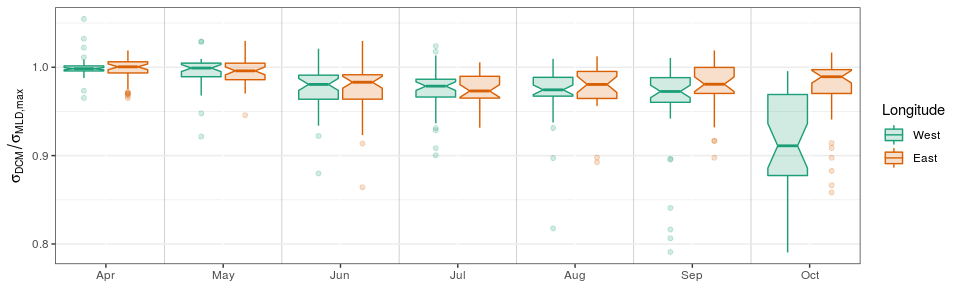
\includegraphics[width=.8\columnwidth]{figs/FIG8.png}
		    \end{figure}
 
	    \end{column}
	  \end{columns}
	  \vskip -5mm
	\end{block}
	

	
      \end{column}
    \end{columns}
    
    % \vspace{2cm}
    % \begin{columns}[T]
    % \end{columns}
    
    
\end{frame}
\end{document}